\documentclass[13pt,oneside]{book}
\usepackage[utf8]{inputenc}
\usepackage{url}
\usepackage{graphicx}

\usepackage{geometry}
\geometry{a4paper, left=20mm, right=20mm, top=20mm, bottom=20mm}
\usepackage[margin=1.2in]{geometry}
\usepackage[toc,page]{appendix}
\usepackage{graphicx}
\usepackage{natbib}
\usepackage{lipsum}
\usepackage{caption}

\begin{document}

\captionsetup[figure]{margin=1.5cm,font=small,labelfont={bf},name={Figure},labelsep=colon,textfont={it}}
\captionsetup[table]{margin=1.5cm,font=small,labelfont={bf},name={Table},labelsep=colon,textfont={it}}
\setlipsumdefault{1}

\begin{titlepage}
\begin{center}
{\LARGE College Of Engineering Trivandrum}\\[3cm]
\linespread{1.2}\huge {\bfseries Application Software Development Lab}\\[3cm]
\linespread{1}

\includegraphics[width=5cm]{img/emblem.jpeg}\\[3cm]
{\Large GOKUL K\\ S5  CSE \\ Roll No:21\\ TVE18CS021 }\\[1cm]


\textit{ }\\[2cm]
Department of Computer Science\\[0.2cm]
\today
\end{center}

\end{titlepage}

\newpage

\begin{frame}{}
    \centering
    \hspace*{-0.5cm}
    $\vcenter{\hbox{
\includegraphics[width=1.5cm]{img/emblem.jpeg}}}$
    $\vcenter{\resizebox{0.95\textwidth}{!}{
        \begin{tabular}{c}
             CS333 - Application Software Development Lab $\cdot$ 2020 $\cdot$   \\
             \hline 
        \end{tabular}
    }}$
\end{frame}
\section*{Cycle 1}
\section*{Expt 5}
\begin{center}
    \Large{Data Constraint and Views}
\end{center}

\section*{Aim}
\large To study about various data constraints and views in SQL.

\section*{Expiriment}
\begin{itemize}
	\item
	\begin{verbatim}
	Create the following tables with given constraints. 
			a. Create a table named Subjects with the given attributes. 
					• Sub_id ( Should not be NULL) 
					• Sub_name (Should not be NULL) 
					• Populate the database. Make sure that all constraints are working properly. 
					Sub_id Sub_name 
					1 Maths 
					2 Physics 
					3 Chemistry 
					4 English 
					i. Alter the table to set Sub_id as the primary key. 
			b. Create a table named Staff with the given attributes. 
					• Staff_id (Should be UNIQUE) 
					• Staff_name 
					• Dept 
					• Age ( Greater than 22) 
					• Salary (Less than 35000) 
					Staff_id Staff_name Dept Age Salary 
					1 John Purchasing 24 30000 
					2 Sera Sales 25 20000 
					3 Jane Sales 28 25000 
					i. Delete the check constraint imposed on the attribute Salary. 
					ii. Delete the unique constraint on the attribute Staff_id. 
			c. Create a table named Bank with the following attributes. 
					• Bank_code (To be set as Primary Key, type= varchar(3) ) 
					• Bank_name (Should not be NULL) 
					• Head_office 
					• Branches (Integer value greater than Zero) 
					i. Make sure that all constraints are working properly. All constraints 
					have to be set after creating the table. 
					Bank_code Bank_name Head_office Branches 
					AAA SIB Ernakulam 6 
					BBB Federal Kottayam 5 
					CCC Canara Trivandrum 3 
					SBT Indian Delhi 7 
			d. Create a table named Branch with the following attributes. 
					• Branch_id (To be set as Primary Key) 
					• Branch_name (Set Default value as ‘New Delhi") 
					• Bank_id (Foreign Key:- Refers to bank code of Bank table) 
					i. Populate the database. Make sure that all constraints are working 
					properly. 
					Branch_id Branch_name Bank_id 
					1 Kottayam CCC 5 Calicut SBT 
					ii. During database population, demonstrate how the DEFAULT 
					Constraint is satisfied. (Insert values with branch as “New Delhi”)
					 iii. Delete the bank with 
					bank code "SBT" and make sure that the 
					corresponding entries are getting deleted from the related tables. 
					iv. Drop the Primary Key using ALTER command 
	\end{verbatim}
Syntax: 	
\begin{verbatim}
	CREATE TABLE IF NOT EXISTS Subjects (
			Sub_id INT NOT NULL,
			Sub_name VARCHAR(10) NOT NULL
	);
	INSERT INTO Subjects
	VALUES
			(1, "Maths"),
			(2, "Physics"),
			(3, "Chemistry"),
			(4, "English");
	ALTER TABLE Subjects
	ADD PRIMARY KEY(Sub_id);
	CREATE TABLE IF NOT EXISTS Staff (
			Staff_id INT NOT NULL UNIQUE,
			Staff_name VARCHAR(10),
			Dept VARCHAR(10),
			Age INT,
			Salary INT,
			CHECK(AGE > 22), 
			CONSTRAINT Staff_Staff_id_key UNIQUE Staff_id,
			CONSTRAINT Staff_Salary_check CHECK(Salary < 35000)
	);
	INSERT Into Staff
	VALUES
			("1","John","Purchasing","24","30000"),
			("2","Sera","Sales","25","20000"),
			("3","Jane","Sales","28","25000");
	ALTER TABLE Staff
	DROP CONSTRAINT Staff_Salary_check;
	ALTER TABLE Staff
	DROP CONSTRAINT Staff_Staff_id_key;
	CREATE TABLE IF NOT EXISTS Bank (
			Bank_code VARCHAR(3),
			Bank_name VARCHAR(10),
			Head_office VARCHAR(10),
			Branches INT
	);
	ALTER TABLE Bank
	ADD CONSTRAINT primary_key PRIMARY KEY (Bank_code);
	ALTER TABLE Bank
	ADD CONSTRAINT branch_office CHECK (Branches > 0);
	INSERT INTO Bank
	VALUES
			("AAA", "SIB", "Ernakulam", 6),
			("BBB", "Federal", "Kottayam", 5),
			("CCC", "Canara", "Trivandrum", 3);
	CREATE TABLE IF NOT EXISTS Branch (
			Branch_id INT,
			Branch_name VARCHAR(10) DEFAULT 'New Delhi',
			Bank_id VARCHAR(3),
			CONSTRAINT Branch_pkey PRIMARY KEY (Branch_id) 
	);
	ALTER TABLE Branch
	ADD CONSTRAINT Branch_Bank_id_fkey 
			FOREIGN KEY (Bank_id) REFERENCES Bank(Bank_code) ON UPDATE CASCADE ON DELETE CASCADE;
	INSERT INTO Branch
	VALUES
			(1, "Kottayam", "CCC"),
			(2, NULL, "AAA");
	INSERT INTO Bank
	VALUES ("SBT", "Indian", "Delhi", 7);
	INSERT INTO Branch
	VALUES (5, "Calicut", "SBT");
	DELETE FROM Bank
	WHERE Bank_code='SBT';
	ALTER TABLE Branch
	DROP CONSTRAINT Branch_pkey;
	INSERT INTO Branch
	VALUES (1, "PPP", "CCC");
	
	\end{verbatim}
	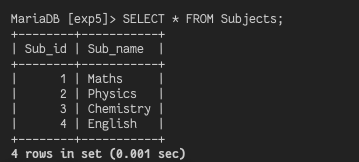
\includegraphics[]{img/p5/ss1.1.png} \\
	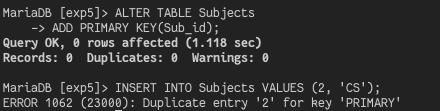
\includegraphics[]{img/p5/ss1.2.png} \\
	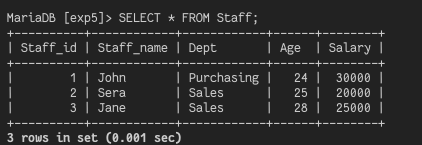
\includegraphics[]{img/p5/ss1.3.png} \\
	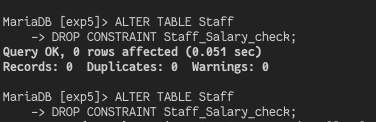
\includegraphics[]{img/p5/ss1.4.png} \\
	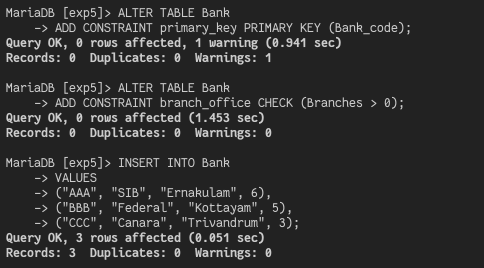
\includegraphics[]{img/p5/ss1.5.png} \\
	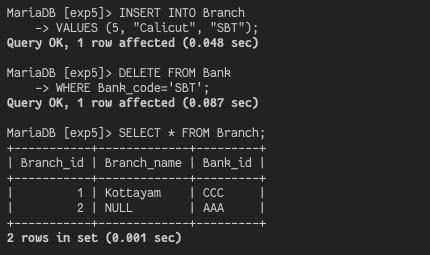
\includegraphics[]{img/p5/ss1.6.png} \\
	
	
	\item
	Create a View named sales\_staff to hold the details of all staff working in sales 
			Department. (Refer to table Staff in question 1(b)) 
	 
	Syntax:
	\begin{verbatim}
	CREATE VIEW sales_staff AS 
			(SELECT * FROM Staff WHERE Dept="SALES");
	SELECT * FROM sales_staff;
	
	\end{verbatim}
	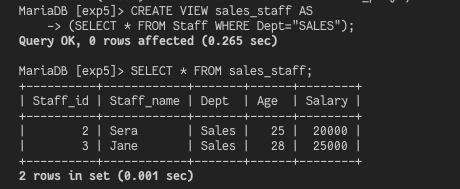
\includegraphics[]{img/p5/ss2.png}
	
	
	\item
	Drop table branch. Create another table named branch and name all the constraints as 
			given below: 
			• Constraint name Column Constraint 
			• Pk branch\_id Primary key 
			• Df branch\_name Default :"New Delhi" 
			• Fk bankid Foreign key/References 
			i. Delete the default constraint in the table ii. Delete the primary key constraint 
	 
	Syntax:
	\begin{verbatim}
	DROP TABLE Branch;
	CREATE TABLE Branch (
			Branch_id INT,
			Branch_name VARCHAR(10) CONSTRAINT Df DEFAULT 'New Delhi',
			Bank_id VARCHAR(3),
			CONSTRAINT Pk PRIMARY KEY (Branch_id),
			CONSTRAINT Fk FOREIGN KEY (Bank_id) REFERENCES Bank (Bank_code) ON UPDATE CASCADE ON DELETE CASCADE
	);
	ALTER TABLE Branch 
	DROP CONSTRAINT Df;
	ALTER TABLE Branch
	DROP CONSTRAINT Pk;
	
	\end{verbatim}
	
	
	\item
	Update the view sales staff to include the details of staff belonging to sales department whose salary is greater than 20000. 
	 
	Syntax:
	\begin{verbatim}
	CREATE OR REPLACE VIEW sales_staff 
	AS (SELECT * FROM Staff WHERE Salary > 20000 AND Dept="Sales");
	
	\end{verbatim}
	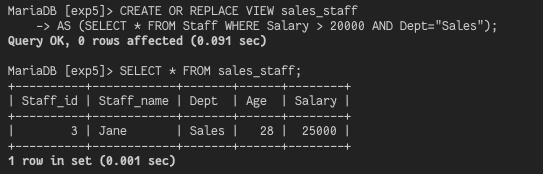
\includegraphics[]{img/p5/ss4.png}
	
	
	\item
	Delete the view sales staff.
	
	Syntax:
	\begin{verbatim}
	DROP VIEW sales_staff;
	\end{verbatim}
	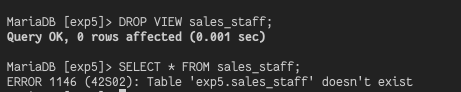
\includegraphics[]{img/p5/ss5.png}
\end{itemize}
\section*{Result}
	The basic SQL for creating and modifying a table is executed and their output
	is verified in a MySQL environment.
\end{document}